\documentclass[11pt]{article}

\usepackage[colorlinks=true]{hyperref}

% This is a toggle for whether the solutions should be included in output of this document
\newif\ifSolutions
%\Solutionsfalse  % this is used to exclude the solutions
\Solutionstrue  % this is used to include the solutions


\usepackage[left=0.8in, right=0.8in, top=0.7in, bottom=1in, includefoot]{geometry}
\usepackage{fancyhdr}
\usepackage{array}
\usepackage{multicol}
\setlength{\parindent}{0mm}
\setlength{\parskip}{5pt}
\usepackage{sectsty}
\allsectionsfont{\sffamily}
\setlength{\headheight}{2cm}
\usepackage{amsmath,amssymb,bm}
\usepackage{booktabs}
\usepackage{graphicx}
\usepackage{color}
\usepackage{cancel}
\usepackage{comment}
\usepackage{hyperref}
\usepackage{subfig}
\usepackage{multirow}
\usepackage{placeins}

% Global definitions
%
% boldface letters
%
%\newcommand{\boldface}[1]{\mathbf{#1}}   % upright
\newcommand{\boldface}[1]{\boldsymbol{#1}}  % italic (slanted)
%
\newcommand{\bfa}{\boldface{a}}
\newcommand{\bfb}{\boldface{b}}
\newcommand{\bfc}{\boldface{c}}
\newcommand{\bfd}{\boldface{d}}
\newcommand{\bfe}{\boldface{e}}
\newcommand{\bff}{\boldface{f}}
\newcommand{\bfg}{\boldface{g}}
\newcommand{\bfh}{\boldface{h}}
\newcommand{\bfi}{\boldface{i}}
\newcommand{\bfj}{\boldface{j}}
\newcommand{\bfk}{\boldface{k}}
\newcommand{\bfl}{\boldface{l}}
\newcommand{\bfm}{\boldface{m}}
\newcommand{\bfn}{\boldface{n}}
\newcommand{\bfo}{\boldface{o}}
\newcommand{\bfp}{\boldface{p}}
\newcommand{\bfq}{\boldface{q}}
\newcommand{\bfr}{\boldface{r}}
\newcommand{\bfs}{\boldface{s}}
\newcommand{\bft}{\boldface{t}}
\newcommand{\bfu}{\boldface{u}}
\newcommand{\bfv}{\boldface{v}}
\newcommand{\bfw}{\boldface{w}}
\newcommand{\bfx}{\boldface{x}}
\newcommand{\bfy}{\boldface{y}}
\newcommand{\bfz}{\boldface{z}}
%
\newcommand{\bfA}{\boldface{A}}
\newcommand{\bfB}{\boldface{B}}
\newcommand{\bfC}{\boldface{C}}
\newcommand{\bfD}{\boldface{D}}
\newcommand{\bfE}{\boldface{E}}
\newcommand{\bfF}{\boldface{F}}
\newcommand{\bfG}{\boldface{G}}
\newcommand{\bfH}{\boldface{H}}
\newcommand{\bfI}{\boldface{I}}
\newcommand{\bfJ}{\boldface{J}}
\newcommand{\bfK}{\boldface{K}}
\newcommand{\bfL}{\boldface{L}}
\newcommand{\bfM}{\boldface{M}}
\newcommand{\bfN}{\boldface{N}}
\newcommand{\bfO}{\boldface{O}}
\newcommand{\bfP}{\boldface{P}}
\newcommand{\bfQ}{\boldface{Q}}
\newcommand{\bfR}{\boldface{R}}
\newcommand{\bfS}{\boldface{S}}
\newcommand{\bfT}{\boldface{T}}
\newcommand{\bfU}{\boldface{U}}
\newcommand{\bfV}{\boldface{V}}
\newcommand{\bfW}{\boldface{W}}
\newcommand{\bfX}{\boldface{X}}
\newcommand{\bfY}{\boldface{Y}}
\newcommand{\bfZ}{\boldface{Z}}

\newcommand{\bfFe}{\boldface{F}_{\text{e}}}
\newcommand{\bfFp}{\boldface{F}_{\text{p}}}
\newcommand{\bfepse}{\pmb{\varepsilon}_{\text{e}}}
\newcommand{\bfepsp}{\pmb{\varepsilon}_{\text{p}}}
\newcommand{\bfeps}{\pmb{\varepsilon}}

%
% boldface greek symbols
%
\newcommand{\bfalpha}{\boldsymbol{\alpha}}
\newcommand{\bfbeta}{\boldsymbol{\beta}}
\newcommand{\bfgamma}{\boldsymbol{\gamma}}
\newcommand{\bfdelta}{\boldsymbol{\delta}}
\newcommand{\bfepsilon}{\pmb{\varepsilon}}
\newcommand{\bfzeta}{\boldsymbol{\zeta}}
\newcommand{\bfeta}{\boldsymbol{\eta}}
\newcommand{\bftheta}{\boldsymbol{\theta}}
\newcommand{\bfkappa}{\boldsymbol{\kappa}}
\newcommand{\bflambda}{\boldsymbol{\lambda}}
\newcommand{\bfrho}{\boldsymbol{\rho}}
\newcommand{\bfmu}{\boldsymbol{\mu}}
\newcommand{\bfnu}{\boldsymbol{\nu}}
\newcommand{\bfpi}{\boldsymbol{\pi}}
\newcommand{\bfxi}{\boldsymbol{\xi}}
\newcommand{\bfsigma}{\boldsymbol{\sigma}}
\newcommand{\bftau}{\boldsymbol{\tau}}
\newcommand{\bfphi}{\boldsymbol{\phi}}
\newcommand{\bfvarphi}{\boldsymbol{\varphi}}
\newcommand{\bfchi}{\boldsymbol{\chi}}
\newcommand{\bfomega}{\boldsymbol{\omega}}
\newcommand{\bfnull}{\boldsymbol{0}}
%
\newcommand{\bfGamma}{\boldsymbol{\Gamma}}
\newcommand{\bfDelta}{\boldsymbol{\Delta}}
\newcommand{\bfTheta}{\boldsymbol{\Theta}}
\newcommand{\bfLambda}{\boldsymbol{\Lambda}}
\newcommand{\bfPi}{\boldsymbol{\Pi}}
\newcommand{\bfXi}{\boldsymbol{\Xi}}
\newcommand{\bfSigma}{\boldsymbol{\Sigma}}
\newcommand{\bfPhi}{\boldsymbol{\Phi}}
\newcommand{\bfChi}{\boldsymbol{\Chi}}
\newcommand{\bfOmega}{\boldsymbol{\Omega}}
\newcommand{\bfnabla}{\boldsymbol{\nabla}}
\newcommand{\laplace}{\boldsymbol{\Delta}}
%
% caligraphic letters
%
\newcommand{\calA}{\mathcal{A}}
\newcommand{\calB}{\mathcal{B}}
\newcommand{\calC}{\mathcal{C}}
\newcommand{\calD}{\mathcal{D}}
\newcommand{\calE}{\mathcal{E}}
\newcommand{\calF}{\mathcal{F}}
\newcommand{\calG}{\mathcal{G}}
\newcommand{\calH}{\mathcal{H}}
\newcommand{\calI}{\mathcal{I}}
\newcommand{\calJ}{\mathcal{J}}
\newcommand{\calK}{\mathcal{K}}
\newcommand{\calL}{\mathcal{L}}
\newcommand{\calM}{\mathcal{M}}
\newcommand{\calN}{\mathcal{N}}
\newcommand{\calO}{\mathcal{O}}
\newcommand{\calP}{\mathcal{P}}
\newcommand{\calQ}{\mathcal{Q}}
\newcommand{\calR}{\mathbb{R}}
\newcommand{\calS}{\mathcal{S}}
\newcommand{\calT}{\mathcal{T}}
\newcommand{\calU}{\mathcal{U}}
\newcommand{\calV}{\mathcal{V}}
\newcommand{\calW}{\mathcal{W}}
\newcommand{\calX}{\mathcal{X}}
\newcommand{\calY}{\mathcal{Y}}
\newcommand{\calZ}{\mathcal{Z}}
% .. define more if needed
%
% double stroke
%
\newcommand{\dsA}{\mathbb{A}}
\newcommand{\dsB}{\mathbb{B}}
\newcommand{\dsC}{\mathbb{C}}
\newcommand{\dsD}{\mathbb{D}}
\newcommand{\dsE}{\mathbb{E}}
\newcommand{\dsF}{\mathbb{F}}
\newcommand{\dsG}{\mathbb{G}}
\newcommand{\dsH}{\mathbb{H}}
\newcommand{\dsI}{\mathbb{I}}
\newcommand{\dsJ}{\mathbb{J}}
\newcommand{\dsK}{\mathbb{K}}
\newcommand{\dsL}{\mathbb{L}}
\newcommand{\dsM}{\mathbb{M}}
\newcommand{\dsN}{\mathbb{N}}
\newcommand{\dsO}{\mathbb{O}}
\newcommand{\dsP}{\mathbb{P}}
\newcommand{\dsQ}{\mathbb{Q}}
\newcommand{\dsR}{\mathbb{R}}
\newcommand{\dsS}{\mathbb{S}}
\newcommand{\dsT}{\mathbb{T}}
\newcommand{\dsU}{\mathbb{U}}
\newcommand{\dsV}{\mathbb{V}}
\newcommand{\dsW}{\mathbb{W}}
\newcommand{\dsX}{\mathbb{X}}
\newcommand{\dsY}{\mathbb{Y}}
\newcommand{\dsZ}{\mathbb{Z}}



\newcommand{\vect}[1]{\mathbf{#1}}
\newcommand{\grvect}[1]{\mbox{\boldmath{$#1$}}}
\newcommand{\perm}{\mbox{{\Huge $\epsilon$}}}
\newcommand{\transvect}[1]{\vect{#1}^{\mbox{\footnotesize T}}}
\newcommand{\invvect}[1]{\vect{#1}^{\mbox{\footnotesize -1}}}
\newcommand{\partderiv}[2]{\frac{\partial #1}{\partial #2}}
\newcommand{\partderivv}[2]{\frac{\partial^2 #1}{\partial #2^2}}
\newcommand{\totalderiv}[2]{\frac{d #1}{d #2}}

\newcommand{\mg}[1]{{\boldsymbol{#1}}}
\newcommand{\mf}[1]{{\mathfrak{#1}}}
\newcommand{\mfb}[1]{{\boldsymbol{\mathfrak{#1}}}}
\newcommand{\ms}[1]{{\mathscr{#1}}}
\newcommand{\mb}[1]{{\mathbf{#1}}}
\newcommand{\mbb}[1]{{\mathbb{#1}}}
\newcommand{\mbbu}[1]{{\underline{\mathbb{#1}}}\vphantom{#1}}
\newcommand{\mbu}[1]{{\underline{\mathbf{#1}}}\vphantom{#1}}
\newcommand{\mgu}[1]{{\underline{\boldsymbol{#1}}}\vphantom{#1}}
\newcommand{\mr}[1]{{\mathrm{#1}}}
\newcommand{\msf}[1]{{\mathsf{#1}}}
\newcommand{\msfb}[1]{{\boldsymbol{\mathsf{#1}}}}

\newcommand{\dotprod}{\stackrel{\scriptscriptstyle \bullet}{}}
\newcommand{\half}{\frac{1}{2}}
\newcommand{\T}{^{\mathsf{T}}} % x^{T}
\newcommand{\mT}{^{\mathsf{-T}}} % x^{-T}
\newcommand{\wass}{\mathsf{wass}}
\newcommand{\eff}{\mathsf{eff}}
\newcommand{\me}{^{\mathrm{-1}}} % x^{-1}
\newcommand{\Rset}{\ensuremath{\mathbb{R}}}
\newcommand{\Kset}{\ensuremath{K}}
\newcommand{\bul}{$\bullet\;$}
%\newcommand{\red}{\mathrm{red}}
\newcommand{\Fe}{\mathbf{F}_\mathbf{e}}
\newcommand{\Fp}{\mathbf{F}_\mathbf{p}}
\def\rel{{\mathrm{rel}}}

%\newcommand{\D}{\displaystyle}
\newcommand{\abs}{\rule[-1cm]{0cm}{1cm}}
\newcommand{\babs}{\rule[-1cm]{0cm}{2cm}}

\newlength{\boxwidth}
\setlength{\boxwidth}{\textwidth}
\addtolength{\boxwidth}{-1cm}

\newcommand\pl{\partial}
\def\dd{\;\!\mathrm{d}}
\def\DD{\;\!\mathrm{D}}
\def\Lin{\R^{d\times d}} 
\def\R{I\!R}
\def\AM{{\mathrm{AM}}}

\def\btheorem{\begin{theorem}}
\def\etheorem{\end{theorem}}
\def\blemma{\begin{lemma}}
\def\elemma{\end{lemma}}
\def\bproposition{\begin{proposition}}
\def\eproposition{\end{proposition}}
\def\bcorollary{\begin{corollary}}
\def\ecorollary{\end{corollary}}
\def\bdefinition{\begin{definition}}
\def\edefinition{\end{definition}}
\def\bexample{\begin{example}}
\def\eexample{\end{example}}
\def\bremark{\begin{remark}}
\def\eremark{\end{remark}}
\def\bproblem#1{\medskip \noindent {\bf #1}\sl \\ }
\def\eproblem{\rm \medskip}
\newcommand{\bma}{ \left( \ba}
\newcommand{\ema}{ \ea \right)}
\newcommand{\set}[2]{\big\{\: #1 \: \big| \: #2 \:\big\} }
\def\cD{\mathcal{D}}
\def\cL{\mathcal{L}}
\def\cG{\mathcal{G}}
\def\cI{\mathcal{I}}
\def\cJ{\mathcal{J}}
\def\ccA{\mathcal{A}}
\def\rmD{\mathrm{D}}
\def\bbQ{\mathbb{Q}}
\def\bbA{\fg{A\!\!\!A}}
\def\fg{\boldsymbol}
\def\mdot{\fg{:}}
\def\vdot{\fg{\cdot}}
\newcommand{\el}{\mathsf{el}}
\def\id{{\bfI}}
\def\eqldef{{\:{\stackrel{\mathrm{def}}{=}}\:}}
\newcommand{\eps}{\varepsilon}
\def\ol{\overline}
\def\wt{\widetilde}
\def\wh{\widehat}
\def\ds{\displaystyle}
\def\ts{\textstyle}
\def\mtr{^\mathrm{-T}}
\def\inh{^\mathrm{inh}}
\DeclareMathOperator{\divv}{div}
\DeclareMathOperator{\grad}{grad}
\DeclareMathOperator{\tr}{tr}
\DeclareMathOperator{\curl}{curl}
\DeclareMathOperator{\Curl}{Curl}
%\DeclareMathOperator{\T}{T}
\DeclareMathOperator{\argmin}{{arg\,min}}
\DeclareMathOperator{\diag}{diag}
\DeclareMathOperator{\trace}{tr}
\DeclareMathOperator{\sign}{sign}
\DeclareMathOperator{\dev}{dev}
\DeclareMathOperator{\cof}{cof}
\DeclareMathOperator{\sym}{sym}
\DeclareMathOperator{\skews}{skw}
\def\Felast{\bfF_\mathbf{\!e}}
\def\Fplast{\bfF_\mathbf{\!p}}
\def\Cplast{\bfC_\mathbf{\!p}}
\def\epselast{\bfeps_\mathbf{\!e}}
\def\epsplast{\bfeps_\mathbf{\!p}}
\def\GLin{\mbox{{\sf GL}$(d)$}}  %{\R^{d\times d}_*}% invertible matrices
\def\Lin{\R^{d\times d}}        % all d times d matrices
\def\reff#1{(\ref{#1})}
\def\red{{\mathrm{red}}}
\def\rep{{\mathrm{rep}}}
\def\cond{{\mathrm{cond}}}
\newcommand{\kopfcolor}{\color{red}}
\newcommand{\er}{\hspace*{4cm}}
\newcommand{\n}{{\rm n}}
\newcommand{\nn}{{\rm n+1}}
\newcommand{\PsiS}{\Psi_\mathrm{S}}
\newcommand{\PsiV}{\Psi_\mathrm{V}}
\newcommand{\PsiI}{\Psi_\mathrm{I}}
\newcommand{\cA}{c_\mathrm{A}}
\newcommand{\cM}{c_\mathrm{M}}

\newcommand{\calAe}{\underset{e=1}{\overset{n_e}{\mathcal{A}}}}
\newcommand{\Grad}{\text{Grad}}
\newcommand{\tcr}{\tau_{\text{crit}}}
\newcommand{\be}{\begin{equation}\nonumber}
\newcommand{\ee}{\end{equation}}
\newcommand{\beq}{\begin{eqnarray}}
\newcommand{\eeq}{\end{eqnarray}}
\newcommand{\bem}{\begin{multline}}
\newcommand{\eem}{\end{multline}}
\newcommand{\ba}{\begin{align}}
\newcommand{\ea}{\end{align}}
\newcommand{\bfzero}{{\fg0}}

\renewcommand{\figurename}{Figure}
\renewcommand{\tablename}{Table}

\newcommand{\fp}[2]{\frac{\partial #1}{\partial #2} }
\newcommand{\LR}{{\qquad \Leftrightarrow \qquad }}
\newcounter{problem}
\newcounter{points}
\newcounter{stretchPoints}

\newcommand{\head}[3]{

\begin{center}
\section*{Homework Set \##1 \ifSolutions Solutions \fi}
assigned: #2\\
due: #3, 11:00 pm\\
in your repo at /cs/cs181j/2015/fall/students/your\_user\_name/cs181j \\
\end{center}
\hrule
\vskip 0.1cm
}

\newcommand{\prob}[1]{\par\vskip 0.5cm \stepcounter{problem}\subsubsection*{Problem \arabic{problem} \ \small (#1 points).}\addtocounter{points}{#1}}
\newcommand{\total}{
\begin{flushright}
\small\par\vskip 0.3cm \textit{total: \arabic{points} points ({\color{blue}+\arabic{stretchPoints} stretch points})}
\end{flushright}
}

\newcommand{\eprob}[2]{\par\vskip 0.5cm \stepcounter{problem}\subsubsection*{Problem \arabic{problem}: #2 \ \small (#1 points).}\addtocounter{points}{#1}}

\newcommand{\estretchprob}[3]{\par\vskip 0.5cm \stepcounter{problem}\subsubsection*{Problem \arabic{problem}: #3 \ \small (#1 points ({\color{blue}+#2 stretch points}) ).}\addtocounter{points}{#1}\addtocounter{stretchPoints}{#2}}


%\endinput

\usepackage{afterpage}
\usepackage{enumerate}

\begin{document}
\sffamily
\pagestyle{fancy}
\renewcommand{\headrulewidth}{0.4pt}
\fancyfoot[C]{\sffamily \thepage{}}
\fancyhead[C]{\vskip 0.7cm \sffamily\footnotesize \textbf{cs181j -- High Performance Computing} \hfill \name\\ Fall 2015 \hfill Harvey Mudd College}

% Convenience function used for including a figure
\newcommand\Figure[3]
{
    \begin{figure}[h!]
        \begin{center}
    \includegraphics[width=#3 in]{#1}
    \caption{\label{fig:#1} {#2}}
    \end{center}
    \end{figure}
}

\newcommand\TwoFigure[7]
{
    \begin{figure}[h!]
        \subfloat[#2]{\includegraphics[width=#7 in]{#1}}
    \hfill
        \subfloat[#4]{\includegraphics[width=#7 in]{#3}}
        \caption{\label{fig:#6}#5}
    \end{figure}
}

\newcommand\TwoFigureVertical[7]
{
    \begin{figure}[h!]
        \subfloat[#2]{\includegraphics[width=#7 in]{#1}}

        \subfloat[#4]{\includegraphics[width=#7 in]{#3}}
        \caption{\label{fig:#6}#5}
    \end{figure}
}


\fancyhead[RL]{}

%\newcommand{\name}{I forgot to change my name}


\head{5}{Wednesday, Oct 7, 2015}{Wednesday, Oct 14, 2015}

Vectorization is an important way in which computers are increasing their throughput. Many people, including almost all sane ones, want the compiler to do their vectorization for them. The purpose of this assignment is for you to learn how to write your own vectorized code using \textbf{intrinsics} as well as to learn to convince the compiler (specifically, its \textbf{autovectorizer}) to do it for you.  Lastly, when the autovectorizer refuses to do something, we'll try to convince \textbf{openmp} to convince the autovectorizer to do it for you.  

You're going to vectorize several problems on this assignment.  In each problem, I have provided the serial versions of each algorithm as well as all the testing logic, timing, and figure-making scaffolding; you should only have to insert code in the \texttt{TODOs}.

Problem 1 involves some simple \textbf{calculations over vectors}, problem 2 is vectorizing a \textbf{scalar integrator} (like, the calculus-1-Riemann-sum style), and problem 3 is vectorizing the calculation of \textbf{Euclidean distances} within a machine learning technique called \href{https://en.wikipedia.org/wiki/K-means_clustering}{k-means clustering}.  By the way, pink text is clickable, and you should click it.

\begin{itemize}
  \item It may not be possible to convince the autovectorizer or the openmp library to vectorize all of these problems - that's part of the \textit{fun}.  It's very important for you to go through the process of trying to convince it, figuring out what type of things they can and can't vectorize, giving up and cursing at them.  The solutions will not have successful autovectorized or openmp versions for some of the problems below.  If you are able to autovectorize something that I couldn't, you'll get super neato awesome points.  If you aren't able to autovectorize something that I couldn't, you don't get marked off. It's kind of a bummer not knowing if you should keep pushing the autovectorizer, but unfortunately that's part of the game.  Yay for compilers!

  \item Information on SSE intrinsics can be found \href{https://software.intel.com/sites/landingpage/IntrinsicsGuide}{here}. Information on autovectorization can be found \href{https://gcc.gnu.org/projects/tree-ssa/vectorization.html}{here}, \href{http://www.slideshare.net/linaroorg/using-gcc-autovectorizer}{here}, and \href{http://locklessinc.com/articles/vectorize/}{here}. Information on trying to get the autovectorizer to tell you what it's thinking can be found \href{https://gcc.gnu.org/onlinedocs/gcc/Debugging-Options.html}{here}, if you search for ``vectorizer''.  I already have set up the Makefiles to output information about autovectorization into \texttt{autovectorization.out.MainX}.

  \item Information on using openmp to vectorize loops can be found \href{http://www.openmp.org/mp-documents/OpenMP4.0.0.pdf}{here}, starting on page 68 or \href{http://moodle.rrze.uni-erlangen.de/moodle/pluginfile.php/10607/mod\_resource/content/1/02%20OpenMP%20in%20a%20Nutshell.pdf}{here}, starting on slide 10.  Also, \href{https://software.intel.com/en-us/videos/performance-essentials-4-openmp-4-vectorization-omp-simd}{this video series} about openmp is good, even though some of the features they describe are not available in GCC.
  
  \item \texttt{shuffler's} architecture was one of the first architectures with \texttt{AVX}.  In typical fashion, the first architectures which support the new specification aren't quite complete - all instructions run but some instructions will serialize into two \texttt{SSE} calls.  In particular, the \texttt{AVX} division and \texttt{sqrt} instructions turn into two \texttt{SSE} calls on \texttt{shuffler}.  As such, where you still close enough to the same answer to not trigger the correctness checks, try using the reciprocal instructions (\texttt{\_mm\_rcp\_ps} and \texttt{\_mm256\_rcp\_ps}) instead of division for full speedup.

  \item The problems will ask you to implement a ``manual'' version and a ``compiler'' version.  For the manual version you can do either \texttt{sse} or \texttt{avx}, and for the compiler version, you can do either \texttt{auto} or \texttt{omp}.  
\end{itemize}

\estretchprob{45}{10}{Vectorizing machine}

In this problem, we'll vectorize some simple calculations over arrays.

\begin{enumerate}[a)]
\item \texttt{sdot} is a level-1 \href{https://en.wikipedia.org/wiki/Basic_Linear_Algebra_Subprograms}{BLAS} function which computes the dot product of two (single-precision) vectors.  Implement the following versions of the \texttt{computeSdot} function in \texttt{Main1\_functions\_sdot.h}:
\begin{itemize}
  \item Implement a \texttt{manual} version.
  \item Implement a \texttt{compiler} version.
  \item (\textit{stretch, 5 points}) \href{http://en.wikipedia.org/wiki/SSE4}{SSE version 4} (termed ``HD Boost'' by Intel's marketing, \textit{*eyeroll*}) introduced \href{http://msdn.microsoft.com/en-us/library/bb514054.aspx}{dot product instructions}.  Implement a manual version which uses either the \texttt{sse} dot product instructions.  Note that we have not talked about masks, so if this is too icky for you, feel free to skip it; I'm trying to give you a flavor for what it's like to try to use random vector instructions in the wild.
  \item (\textit{stretch, 5 points}) Now that we're doing our flops faster, we may be even more worried about memory access and keeping the cruncher fed.  Read about the \texttt{\_mm\_prefetch} instruction (perhaps \href{http://lwn.net/Articles/255364/}{here}, which is an excerpt from the highly-recommended Ulrich Drepper's ``What every programmer should know about memory'') and find an appropriate prefetch distance to make a prefetched \texttt{SSE} version.
\end{itemize}
The python script will plot the speedup of all flavors, and the graph is included here.  Comment on your results.

\ifSolutions
\textbf{Solution:}

{
  \begin{center}
  
\includegraphics[width=7 in]{figures/Main1_sdot_shuffler}
  \end{center}
}

\fi

\item Implement the following versions of the \texttt{computeFixedPolynomial} function (which calculates a fixed polynomial $y[i] = c_0 + c_1x + c_2x^2 + c_3x^3$) in \texttt{Main1\_functions\_fixedPolynomial.h}:
\begin{itemize}
  \item Implement a \texttt{manual} version.
  \item Implement a \texttt{compiler} version.
\end{itemize}
Plot the speedups that you achieve as a function of vector size for all flavors of \texttt{computeFixedPolynomial} that you implemented.  Comment on your results.

\ifSolutions
\textbf{Solution:}

{
  \begin{center}
  
\includegraphics[width=7 in]{figures/Main1_fixedPolynomial_shuffler}
  \end{center}
}

\fi

\item Spot the bug!  How does the following code lead to a segmentation fault?
\begin{verbatim}
for (index = 0; index < x.size() - 100; index+=8) {
   simdVector = _mm256_load_ps(&x[index + 96])
}
\end{verbatim}

\ifSolutions
\textbf{Solution:}

\fi

\item In many numerical techniques such as finite difference, you have to do operations on arrays of the same size, but with offset indices.  We'll use the following loop to model this type of computation:
\begin{verbatim}
  for (unsigned int i = 0; i < size; ++i)
    w[i] = a * x[i] * y[(i + 16)%size] / (b * z[(i + size - 8)%size]);
\end{verbatim}
Assume that \texttt{size} $> 16$ and \texttt{z[i]} $> 0$. Implement the following versions of the \texttt{computeOffsets} function in \texttt{Main1\_functions\_offsets.h}:
\begin{itemize}
  \item First, mods are expensive, so re-implement this algorithm in the \texttt{scalarNoMod} flavor such that use of mods is minimized.  Minimize or eliminate your use of mods in all following versions.
  \item Implement a \texttt{manual} version.
  \item Implement a \texttt{compiler} version.
\end{itemize}
Plot the speedups that you achieve as a function of vector size and comment on your results.

\ifSolutions
\textbf{Solution:}

{
  \begin{center}
  
\includegraphics[width=7 in]{figures/Main1_offsets_shuffler}
  \end{center}
}

\fi

\item Implement the following versions of the \texttt{computeTaylorExponential} function (which calculates \texttt{exp} using a Taylor series, like from homework 0) in \texttt{Main1\_functions\_taylorExponential.h}:
\begin{itemize}
  \item Implement a \texttt{manual} version.
  \item Implement a \texttt{compiler} version.
\end{itemize}
Plot the speedups that you achieve as a function of vector size and comment on your results.

\ifSolutions
\textbf{Solution:}

{
  \begin{center}
  
\includegraphics[width=7 in]{figures/Main1_taylorExponential_shuffler}
  \end{center}
}

\fi

\item Overall, what do you observe about the performance you found?  What surprises you?  What makes sense?  What types of things could be auto- or omp-vectorized?

\ifSolutions
\textbf{Solution:}

\fi

\end{enumerate}

\vfill

\afterpage{\clearpage}










\eprob{15}{Crossing Vectors with Scalar (integration)}

In this problem, we'll vectorize scalar integration, which does calculations without memory accesses.

\begin{enumerate}[a)]
\item Implement the following versions of the \texttt{integrateSqrt} function in \texttt{Main2\_functions\_sqrt.h}:
\begin{itemize}
  \item Implement a \texttt{manual} version.
  \item Implement a \texttt{compiler} version.
\end{itemize}
Plot the speedups that you achieve as a function of vector size and comment on your results.

\ifSolutions
\textbf{Solution:}

{
  \begin{center}
  
\includegraphics[width=7 in]{figures/Main2_sqrt_shuffler}
  \end{center}
}

\fi

\item Implement the following versions of the \texttt{integrateFixedPolynomial} function in \\ \texttt{Main2\_functions\_fixedPolynomial.h}:
\begin{itemize}
  \item Implement a \texttt{manual} version.
  \item Implement a \texttt{compiler} version.
\end{itemize}
Plot the speedups that you achieve as a function of vector size and comment on your results.

\ifSolutions
\textbf{Solution:}

{
  \begin{center}
  
\includegraphics[width=7 in]{figures/Main2_fixedPolynomial_shuffler}
  \end{center}
}

\fi
\end{enumerate}

\afterpage{\clearpage}
\newpage








\eprob{20}{k-means Clustering (and D means Done)}

{
  \begin{figure}[ht]
    \subfloat[Step 1]{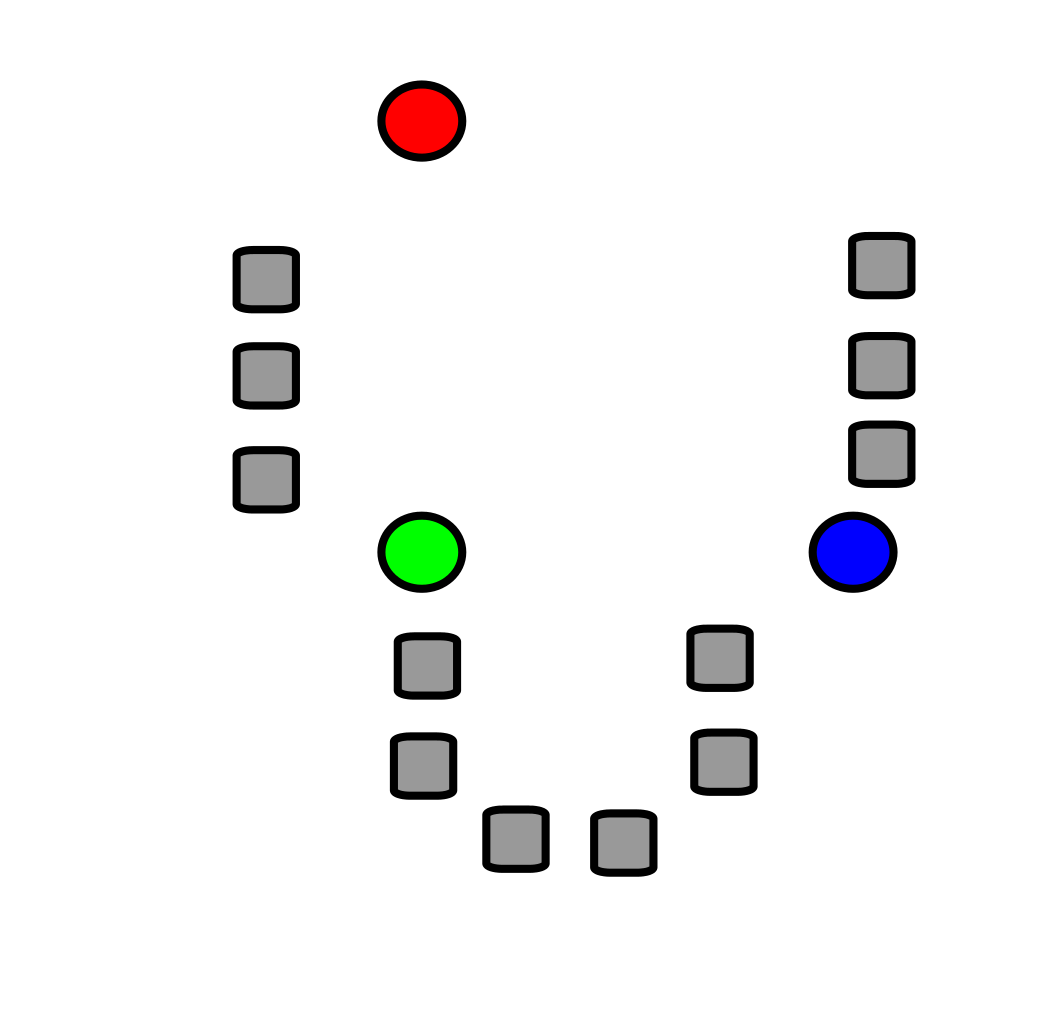
\includegraphics[width=1.5 in]{KMeansExample_Step1}}
    \hfill
    \subfloat[Step 2]{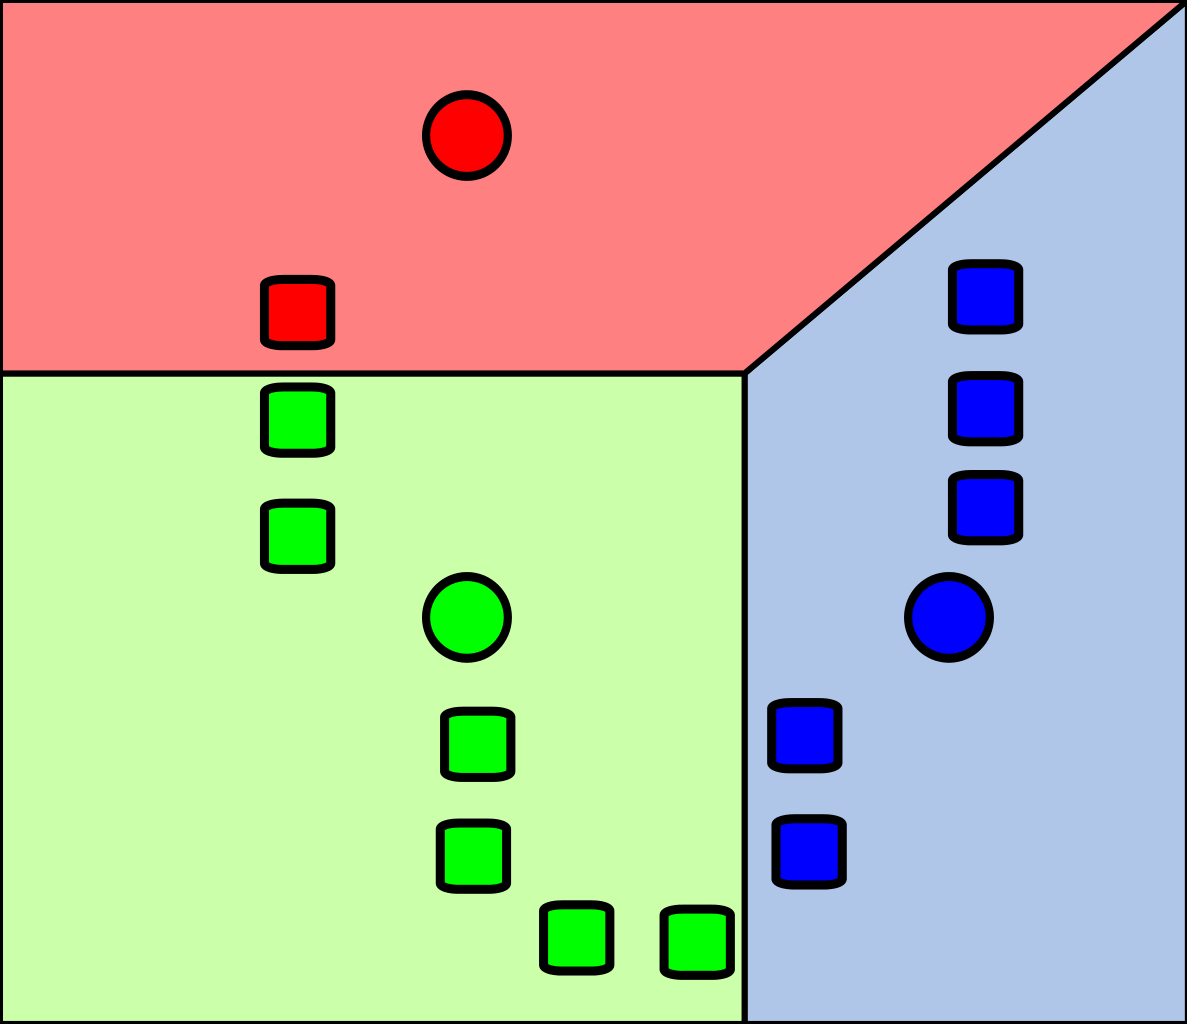
\includegraphics[width=1.5 in]{KMeansExample_Step2}}
    \hfill
    \subfloat[Step 3]{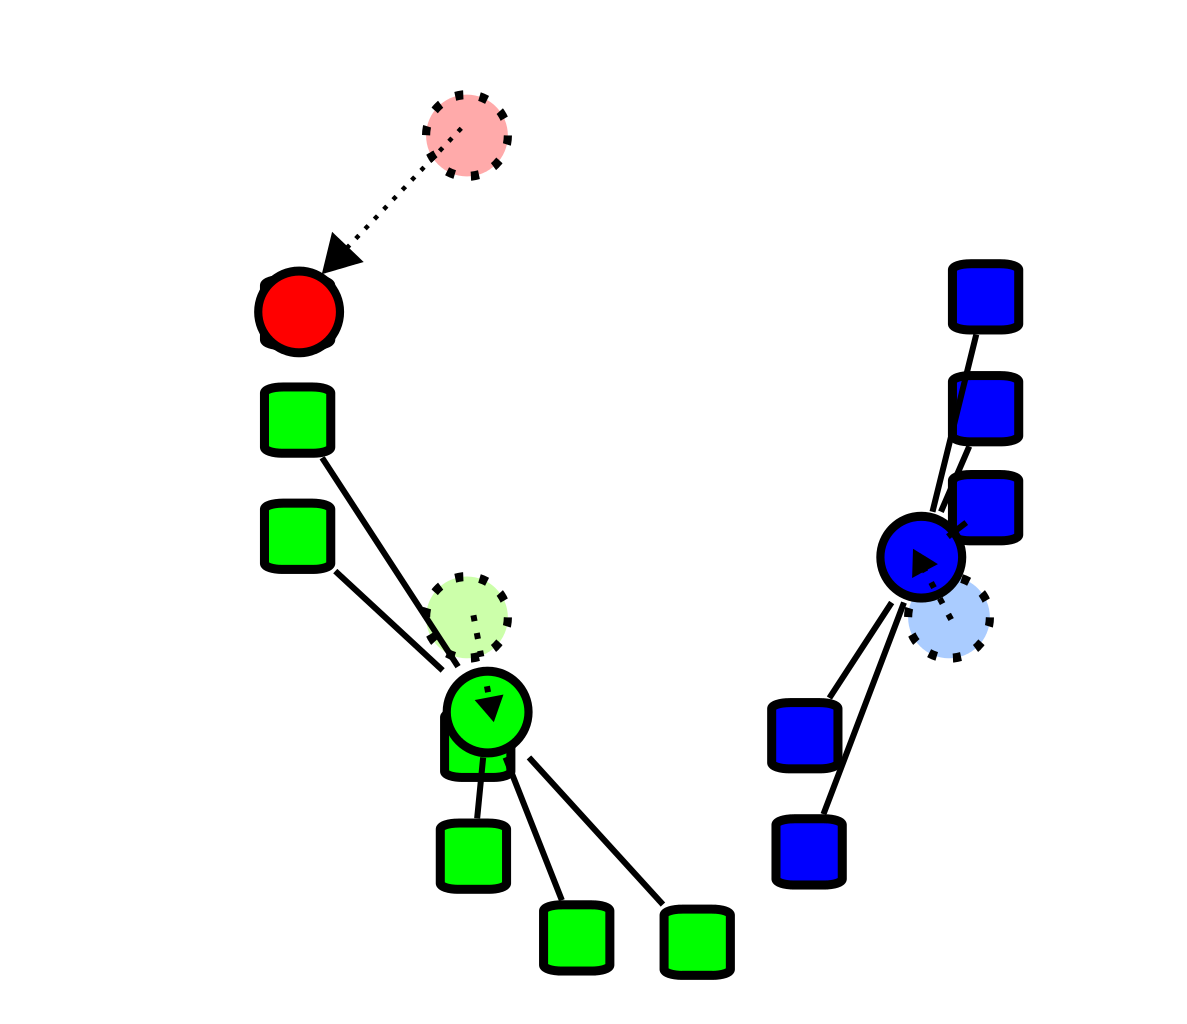
\includegraphics[width=1.5 in]{KMeansExample_Step3}}
    \hfill
    \subfloat[Step 4]{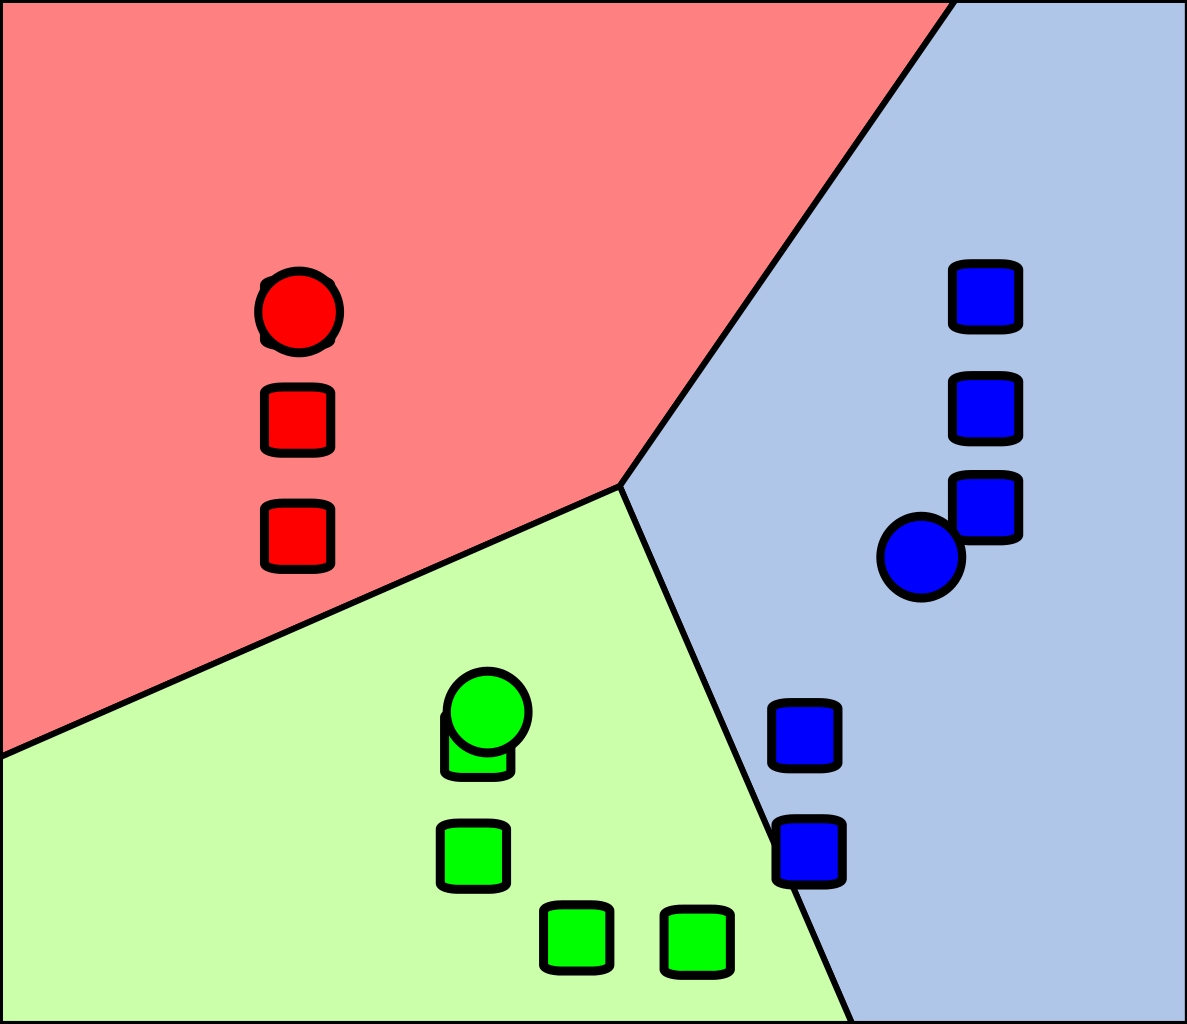
\includegraphics[width=1.5 in]{KMeansExample_Step4}}
    \caption{\label{fig:KMeansClustering} Steps for performing k-means clustering.  Steps 2-4 are repeated until convergence (or a maximum number of iterations is performed)}
  \end{figure}
}

\href{https://en.wikipedia.org/wiki/K-means_clustering}{k-means clustering} is an algorithm that we will revisit a couple more times in the semester after this because the algorithm is straight-forward and lends itself well to various strategies for reducing runtime.  The steps are summarized in figure \ref{fig:KMeansClustering} and are outlined below:

\begin{verbatim}
initialize centroids to random positions

for each iteration
  zero out nextCentroids
  zero out nextCentroidCounts
  for each point
    indexOfClosestCentroid = determine index of closest centroid
    nextCentroids[indexOfClosestCentroid] += point
    ++nextCentroidCounts[indexOfClosestCentroid]

  for i from 0 to numberOfCentroids
    centroids[i] = nextCentroids[i] / nextCentroidCounts[i]
    nextCentroids[i] = zero
    nextCentroidCounts[i] = 0
\end{verbatim}

We'll explore a range of number of points (say from 1,000 to 100,000) as well as a range of number of centroids (say from 5 to 200).  The specific calculation to be vectorized will be finding the nearest centroid for a given point, which means 5 to 200 (squared) distance calculations and comparisons.  In order to make these calculations easily vectorizable, the centroids locations are stored in ``structure of arrays'' format.

\texttt{Main0.cc} has an example of finding the index of the minimum value in a vector, and you should essentially copy and paste helpful pieces of that example to use here.  Instead of trying to find the index of the minimum value in a vector, here you're trying to find the index of the minimum value of numbers you calculate.

Vectorize the k-means calculation and include here the plot of the speedup versus the number of points and number of centroids.  Comment on your results.

\ifSolutions

\textbf{Solution:}

{
  \begin{center}
  
\includegraphics[width=5 in]{figures/KMeans_speedup_shuffler}
  \end{center}
}


\fi

\vfill



\estretchprob{0}{20}{Foggy Vector Libraries}

Vectorization is great and all, but there are some things that you can't do with intrinsics or autovectorization, such as \texttt{exp}, \texttt{sin}, \texttt{pow}, and friends.  There are several vector math libraries that provide this type of functionality (and, conveniently, abstract away all of the nasty \_mm547 nonsense!); the one I want you to explore here is Agner Fog's \href{http://www.agner.org/optimize/vectorclass.pdf}{Vector Class Library}.  Choose an interesting function that you can't compute using intrinsics, calculate it for many inputs using Agner's vector class and with the normal scalar function, and plot your speedup versus vector size.

\vfill




\eprob{15}{Back to the Real World}

Provide short (but sufficient) answers to the following prompts:

\begin{enumerate}[a)]
\item Explain as you would to a ``non-technical'' friend of yours (who knows essentially nothing about computer architecture) the difference between using scalar registers and vector registers.

\ifSolutions
\textbf{Solution:}

\fi

\item How would you answer a lab-mate who asks you ``how do I vectorize my code?''

\ifSolutions
\textbf{Solution:}

\fi

\item There are few things that people like to stick their head in the sand and ignore more \textit{enthusiastically} than vectorization.  Pretend that another lab-mate tells you ``The compiler will do it way better than you ever can and it already does it all automagically anyways''.  How would you respond?

\ifSolutions
\textbf{Solution:}

\fi

\item The peak flops rate possible doubled from the processor before Sandy Bridge (``Nehalem'') to Sandy Bridge because of the introduction of 8-wide AVX SIMD registers.  Yet another lab-mate of yours is considering upgrading their processor from Nehalem to Sandy Bridge to take advantage of this increase in speed and they ask you if it's a good idea.  What would you tell them?

\ifSolutions
\textbf{Solution:}

\fi

\end{enumerate}

\eprob{5}{Feedback}

\begin{enumerate}[a)]
\item How much total time did you spend on this assignment?
\item Of the total time, how much total time did you spend ``flailing'' on little annoying things that are not the main point of the assignment?
\item Of the total time, how much total time did you spend on stretch problems?
\item Did you work with anyone closely on this assignment?
\item Did you have any ``aha'' moments where something clicked?  If so, on what problems or parts?
\item Can you give me any feedback on this assignment?
\item Fill out the mid-semester feedback survey found \href{https://docs.google.com/forms/d/1BtXfvcB9IVBBUworBuqiLIwri6lTcLw-NqEYhr5oNBQ/viewform?usp=send_form}{here}.  I know it's hard, but please try to comment on the class in general and not this specific assignment.
\end{enumerate}

\vskip 1cm
\total


\end{document}

todo: triple the length of the next homework assignment.
